\newpage
\section{ISO/IEC 9126}

\label{ISO/IEC 9126}
\begin{figure}[h]
\centering
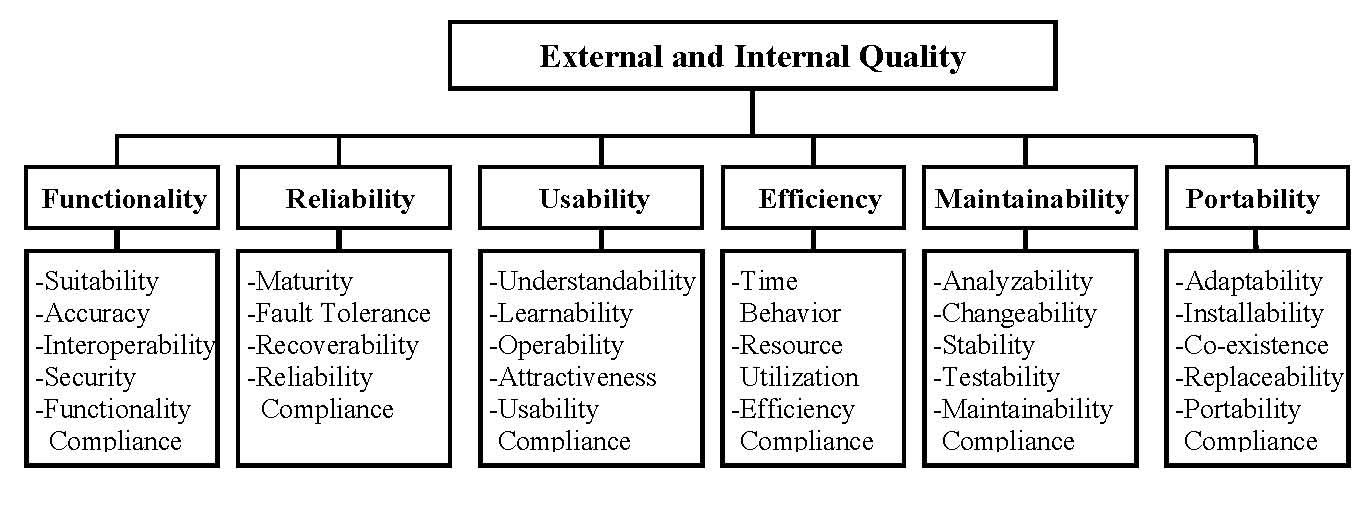
\includegraphics[scale=0.3,keepaspectratio]{9126.png}
\caption{ISO/IEC 9126}
\end{figure}
\FloatBarrier

Lo standard \textit{ISO/IEC 9126}\ped{G} è stato redatto con lo scopo di descrivere quali sono gli obiettivi qualitativi che deve avere un prodotto software. Questi vengono suddivisi in 3 aree tematiche diverse:
\begin{itemize}
\item\textbf{Qualità esterna}: rappresenta la qualità del software nel momento in cui esso viene eseguito e testato;
\item\textbf{Qualità interna}: rappresenta la qualità del software per quanto riguarda le sue caratteristiche implementative, durante le fasi di progettazione e codifica; 
\item\textbf{Qualità in uso}: rappresenta la qualità del software dal punto di vista del cliente che lo sta utilizzando.
\end{itemize}

Poiché non avremo la possibilità di testare la qualità in uso del prodotto, il \textit{team}\ped{G} ha deciso di concentrarsi solamente sulla qualità interna ed esterna. \\ Lo standard delinea sei macro-obbiettivi qualitativi, i quali sono suddivisi a loro volta in sotto caratteristiche specifiche:
\begin{itemize}
\item\textbf{Funzionalità}: capacità del prodotto di fornire tutte le funzioni che sono state individuate attraverso l'\textit{Analisi dei Requisiti}.
\begin{itemize}
\item\textbf{Adeguatezza}: le funzionalità fornite devono essere conformi rispetto le aspettative;
\item\textbf{Accuratezza}: il prodotto deve fornire i risultati attesi, con il livello di precisione richiesto;
\item\textbf{Interoperabilità}: il prodotto deve poter interagire ed operare con uno o più sistemi specifici;
\item\textbf{Sicurezza}: il prodotto deve proteggere le informazioni e i dati da accessi e modifiche non autorizzati.
\item\textbf{Conformità di funzionalità}: il prodotto deve aderire a standard, regole e convenzioni inerenti alla funzionalità;
\end{itemize}
\item\textbf{Affidabilità}: capacità del prodotto software di svolgere correttamente le sue funzioni durante il suo utilizzo, anche nel caso in cui si presentino situazioni anomale.
\begin{itemize}
\item\textbf{Maturità}: il prodotto deve evitare che si verifichino malfunzionamenti o che vengano prodotti risultati non corretti;
\item\textbf{Tolleranza agli errori}: nel caso in cui si presentino degli errori, dovuti a guasti o ad un uso scorretto dell'applicativo, questi devono essere gestiti in modo da mantenere alto il livello di prestazione;
\item\textbf{Recuperabilità}: il prodotto deve essere in grado di ristabilire un
adeguato livello di prestazioni e di recuperare i dati rilevanti in seguito a errori o malfunzionamenti;
\item\textbf{Conformità di affidabilità}: il prodotto deve aderire a standard, regole e convenzioni inerenti all'affidabilità.
\end{itemize}
\item\textbf{Usabilità}: capacità del prodotto di essere facilmente comprensibile e attraente in ogni sua parte per qualsiasi utente che lo andrà ad utilizzare.
\begin{itemize}
\item\textbf{Comprensibilità}: l'utente deve essere in grado di riconoscerne le funzionalità offerte dal software e deve comprenderne le modalità di utilizzo per riuscire a raggiungere i risultati attesi;
\item\textbf{Apprendibilità}: deve essere data la possibilità all'utente di imparare ad utilizzare l'applicazione senza troppo impegno;
\item\textbf{Operabilità}: le funzionalità presenti devono essere coerenti con le aspettative dell'utente;
\item\textbf{Attrattiva}: il software deve essere piacevole per chi ne fa uso;
\item\textbf{Conformità di usabilità}: il prodotto deve aderire a standard, regole e convenzioni inerenti all'usabilità.
\end{itemize}
\item\textbf{Efficienza}: capacità di eseguire le funzionalità offerte dal software nel minor tempo possibile utilizzando al tempo stesso il minor numero di risorse possibili.
\begin{itemize}
\item\textbf{Comportamento rispetto al tempo}: per svolgere le sue funzioni il software deve fornire adeguati tempi di risposta ed elaborazione;
\item\textbf{Utilizzo delle risorse}: il software quando esegue le sue funzionalità deve utilizzare un appropriato numero e tipo di risorse;
\item\textbf{Conformità di efficienza}: il prodotto deve aderire a standard, regole e convenzioni inerenti all'efficienza.
\end{itemize}
\item\textbf{Manutenibilità}: capacità del prodotto di essere modificato, tramite correzioni, miglioramenti o adattamenti del software a cambiamenti negli ambienti, nei requisiti e nelle specifiche funzionali.
\begin{itemize}
\item\textbf{Analizzabilità}: il software deve consentire una rapida identificazione delle possibili cause di errori e malfunzionamenti;
\item\textbf{Modificabilità}: il prodotto originale deve permettere eventuali cambiamenti in alcune sue parti;
\item\textbf{Stabilità}: non devono insorgere effetti indesiderati in seguito a modifiche effettuate sul software;
\item\textbf{Testabilità}: il software deve poter essere facilmente testato per validare le modifiche effettuate;
\item\textbf{Conformità di manutenibilità}: il prodotto deve aderire a standard, regole e convenzioni inerenti alla manutenibilità.
\end{itemize}
\item\textbf{Portabilità}: capacità del software di poter essere utilizzato su diversi ambienti.
\begin{itemize}
\item\textbf{Adattabilità}: il prodotto deve adattarsi a tutti quegli ambienti di lavoro nei quali è stato previsto un suo utilizzo, senza dover apportare modifiche allo stesso;
\item\textbf{Installabilità}: il software deve poter essere installato in determinati ambienti di lavoro;
\item\textbf{Coesistenza}: il prodotto può coesistere in ambienti comuni
con altri software, condividendo risorse comuni;
\item\textbf{Sostituibilità}: l'applicativo deve poter sostituire un altro software che ha lo stesso scopo e lavora nel medesimo ambiente;
\item\textbf{Conformità di portabilità}: il prodotto deve aderire a standard, regole e convenzioni inerenti alla portabilità.
\end{itemize}
\end{itemize}	